%\textcolor{red}{\textbf{!! CAUTION : Efficiency numbers look old. Numbers in AN do not agree with
%/smurf/dlevans/Efficiencies/V00-02-09/HWW\_Electron\_V00-02-09\_Moriond\_V1\_NM1Eff\_ID/summary.txt, 
%but they are from Moriond\_V0. Should replace them. !!}}  


%%%%%%%%%%%%%%%%%%%%%%%%%%%%%%%%%%%%%%%%%%%%%%%%%%%%%%%%%%%%%%%%%%%%%%%%%%%%%%%%%%%%%%%%%%
\section{Lepton Efficiency}

In collisions events are recorded when the two leptons pass trigger requirements. 
Thus, per event trigger efficiency needs to be measured using data. 
To select identified and isolated leptons from Higgs events, we require 
that each lepton meet strict offline criteria. To account for the possible difference
of offline selection efficiencies in simulation and data, we need to measure it 
in simultion and data separately and apply a scale factors
($\epsilon_{data}/\epsilon_{simulation}$) to simulation. 

The efficiencies are measured using Tag-And-Probe method [ref]. We use 
$Z/\gamma^* \rightarrow e^+e^-$ or $Z/\gamma^* \rightarrow \mu^+\mu^-$ events 
passing single-lepton trigger to select unbiased, identified and isolated prompt leptons.  
One lepton which is called "tag" is required to pass the single lepton trigger 
requirement and the full offlince selection. By requiring full selection on the tag, 
we can enhance the purity of the sample. The other lepton which is called 
"probe" is required to pass a set of selection criteria that enhances the purity 
of sample while leaving the crieteria under study unbiased. The fact that tag 
passed sigle-lepton trigger guarantees that the probe is not biased by trigger. 
Both legs can be used as a tag in offline efficiency measurement while only 
can one of them be in trigger efficiency measurement due to the correlation 
between two offlie lepton objects in double-lepton triggers. 

The offline selection efficiency is composed of identification(ID) and isolation(ISO) parts. 
We use N-1 method where ID and ISO efficiencies are measured with respect to the other 
and multiplied afterwards. When measuring efficiency of ID part ($\epsilon_{ID}$) 
probe is required to pass full isolation requirement and when measuring efficiency of 
ISO part ($\epsilon_{ISO}$) probe is required to pass full identification requirement. 
\textcolor{red}{mention that eff is measured as a function of pT and eta of lepton}   
The possible bias due to correlation of the two measurements 
is estimated by comparing efficiencies measured by N-1 method and combined measurement 
of ID+ISO  efficiency in simulation. The difference which ranges from xx to yy depending 
on the kinemtic bins of a lepton is assigned as systematic uncertainty of the method. 
\textcolor{red}{What are the other systematics? For electron, systematics to 
electron reconstruction efficiency(prob for a SC to be matched to a ECAL-driven 
GSF electron), 100 +/- 2\% (measured with 2011 data). In the code, there are 
2 \% and 1.5 \% for electron and muon, repectively. Are they from 
reconstruction efficiency and other ones are negligible compared to these values?} 

Requiring tight selections to tag and using N-1 method gives high-purity sample 
of $Z/\gamma^*$ events in data. However, there are residual contributions from 
non-prompt leptons from W+jets and QCD events especially at low $p_T$ bins. 
Thus, we extract yields by fitting the \mll~distribution of the tag and probe pair
with Gaussian $+$ exponential $\times$ error function. The Gaussian function which 
is for $Z/\gamma^*$ invariant mass peak is modeled by simulation and 
gaussian smearing is applied to account for difference in lepton momentum resolutions
between data and simulation. 
\textcolor{red}{I don't believe this is true. Looking at the plots with fitted shapes, 
it seems that there are more than one fit function. need to check in the code.}
The exponential $\times$ error function is for backgrounds.
To allow enough sidebands for backgrounds, \mll~range is chosen to be 
$60~\GeV < \mll < 120~\GeV$. In case of simulation, efficiencies are calculated by 
counting events in $81~\GeV < \mll < 101~\GeV$. In simulation, to select  
leptons from $Z/\gamma^*$ only (=to remove mis-recontructed leptons), the dR between 
probe and the closest, same flavor, generator-level lepton after final-state-radiation(FSR)
is required to be within 0.2.

The data/simulation efficiency scale factors per event are then calculated by 
multiplying per lepton efficiencies measured in data and simulation, 
\begin{equation} 
\epsilon_{offline}^{event} 
= 
\epsilon_{ID}^{lepton1} \times \epsilon_{ISO}^{lepton1}   
\times \epsilon_{ID}^{lepton2} \times \epsilon_{ISO}^{lepton2}.   
\end{equation} 
The trigger efficiency($\epsilon_{trigger}$) is measured with respect to the full 
offline selection. Finally, simulation events are corrected by applying the 
offline selection scale factor and trigger efficiency, 
\begin{equation} 
\frac{\epsilon_{offline, MC}^{event}}{\epsilon_{offline, MC}^{event}} 
\times \epsilon_{trigger}. 
\end{equation} 



%%%%%%%%%%
\subsection{Electron Selection Efficiency}

Electron efficiency is composed of two factors, recontruction efficiency and 
selection efficiency. The reconstruction efficiency is the probability for a 
super-cluster energy deposit to be matched to a reconstructed ECAL-driven 
GSF electron. For thie analysis, we use the result measured with 2011 data   
because new measurement has not made with the full 2012 data sample[ref]. 
\textcolor{red}{Really no new study?}. The efficency is measured as a function 
of \pt~and \Eta~of a lepton. From the study, we assume that the reconstruction 
efficiency for an electron is unity with uncertainty at the level of 2 \%.

%
\begin{table}[!htp]
\begin{center}
\begin{tabular}{c|c|c|c|c}
\hline & $ 0 < |\eta| < 0.8$ & $ 0.8 < |\eta| < 1.479$ & $ 1.479 < |\eta| < 2 $ & $ 2 < |\eta| < 2.5 $  \\
\hline
\multicolumn{5}{c} {N-1 Efficiencies in data} \\
\hline
$ 10 < p_T <  15$ & $0.3289 \pm 0.0049$ & $0.4353 \pm 0.0046$ & $0.1551 \pm 0.0040$ & $0.1059 \pm 0.0026$  \\
$ 15 < p_T <  20$ & $0.5981 \pm 0.0026$ & $0.6330 \pm 0.0028$ & $0.3140 \pm 0.0033$ & $0.2379 \pm 0.0030$  \\
$ 20 < p_T <  30$ & $0.7208 \pm 0.0009$ & $0.7457 \pm 0.0010$ & $0.5147 \pm 0.0011$ & $0.4609 \pm 0.0021$  \\
$ 30 < p_T <  40$ & $0.8293 \pm 0.0002$ & $0.8481 \pm 0.0004$ & $0.6780 \pm 0.0015$ & $0.5962 \pm 0.0015$  \\
$ 40 < p_T <  50$ & $0.8623 \pm 0.0004$ & $0.8840 \pm 0.0005$ & $0.7558 \pm 0.0007$ & $0.6573 \pm 0.0009$  \\
$ 50 < p_T < 7000$ & $0.8745 \pm 0.0004$ & $0.8936 \pm 0.0005$ & $0.7859 \pm 0.0012$ & $0.6891 \pm 0.0015$  \\
\hline
\multicolumn{5}{c} {N-1 Efficiencies in simulation} \\
\hline
$ 10 < p_T <  15$ & $0.4583 \pm 0.0055$ & $0.5405 \pm 0.0053$ & $0.2267 \pm 0.0058$ & $0.1890 \pm 0.0056$  \\
$ 15 < p_T <  20$ & $0.6671 \pm 0.0030$ & $0.7126 \pm 0.0031$ & $0.3904 \pm 0.0045$ & $0.3426 \pm 0.0047$  \\
$ 20 < p_T <  30$ & $0.7594 \pm 0.0010$ & $0.7943 \pm 0.0011$ & $0.5762 \pm 0.0019$ & $0.5090 \pm 0.0021$  \\
$ 30 < p_T <  40$ & $0.8492 \pm 0.0005$ & $0.8797 \pm 0.0005$ & $0.7215 \pm 0.0010$ & $0.6291 \pm 0.0012$  \\
$ 40 < p_T <  50$ & $0.8774 \pm 0.0004$ & $0.9091 \pm 0.0004$ & $0.7843 \pm 0.0007$ & $0.6915 \pm 0.0010$  \\
$ 50 < p_T < 7000$ & $0.8893 \pm 0.0007$ & $0.9169 \pm 0.0007$ & $0.8039 \pm 0.0013$ & $0.7149 \pm 0.0017$  \\
\hline
\multicolumn{5}{c} {Simulation-to-data scale factors} \\
\hline
$ 10 < p_T <  15$ & $0.7177 \pm 0.0138$ & $0.8053 \pm 0.0117$ & $0.6842 \pm 0.0249$ & $0.5602 \pm 0.0214$  \\
$ 15 < p_T <  20$ & $0.8966 \pm 0.0056$ & $0.8882 \pm 0.0055$ & $0.8045 \pm 0.0126$ & $0.6943 \pm 0.0128$  \\
$ 20 < p_T <  30$ & $0.9491 \pm 0.0017$ & $0.9388 \pm 0.0019$ & $0.8933 \pm 0.0035$ & $0.9056 \pm 0.0056$  \\
$ 30 < p_T <  40$ & $0.9766 \pm 0.0006$ & $0.9641 \pm 0.0007$ & $0.9396 \pm 0.0024$ & $0.9477 \pm 0.0030$  \\
$ 40 < p_T <  50$ & $0.9828 \pm 0.0006$ & $0.9724 \pm 0.0007$ & $0.9637 \pm 0.0013$ & $0.9507 \pm 0.0018$  \\
$ 50 < p_T < 7000$ & $0.9834 \pm 0.0009$ & $0.9746 \pm 0.0009$ & $0.9776 \pm 0.0021$ & $0.9639 \pm 0.0032$  \\
\end{tabular}
\caption{HWW Electron V00-02-09 Moriond jae NM1Eff ID}
\label{tab:eff_electron_id}
\end{center}
\end{table}

\begin{table}[!htp]
\begin{center}
\begin{tabular}{c|c|c|c|c}
\hline & $ 0 < |\eta| < 0.8$ & $ 0.8 < |\eta| < 1.479$ & $ 1.479 < |\eta| < 2 $ & $ 2 < |\eta| < 2.5 $  \\
\hline
\multicolumn{5}{c} {N-1 Efficiencies in data} \\
\hline
$ 10 < p_T <  15$ & $0.7827 \pm 0.0042$ & $0.7973 \pm 0.0029$ & $0.8009 \pm 0.0199$ & $0.8546 \pm 0.0110$  \\
$ 15 < p_T <  20$ & $0.8167 \pm 0.0007$ & $0.8360 \pm 0.0034$ & $0.8155 \pm 0.0145$ & $0.8776 \pm 0.0041$  \\
$ 20 < p_T <  30$ & $0.8798 \pm 0.0011$ & $0.8815 \pm 0.0007$ & $0.8787 \pm 0.0017$ & $0.9246 \pm 0.0091$  \\
$ 30 < p_T <  40$ & $0.9391 \pm 0.0000$ & $0.9398 \pm 0.0007$ & $0.9337 \pm 0.0006$ & $0.9598 \pm 0.0004$  \\
$ 40 < p_T <  50$ & $0.9710 \pm 0.0001$ & $0.9721 \pm 0.0002$ & $0.9704 \pm 0.0002$ & $0.9802 \pm 0.0002$  \\
$ 50 < p_T < 7000$ & $0.9816 \pm 0.0002$ & $0.9815 \pm 0.0008$ & $0.9815 \pm 0.0003$ & $0.9873 \pm 0.0004$  \\
\hline
\multicolumn{5}{c} {N-1 Efficiencies in simulation} \\
\hline
$ 10 < p_T <  15$ & $0.7724 \pm 0.0061$ & $0.8015 \pm 0.0052$ & $0.7856 \pm 0.0109$ & $0.8516 \pm 0.0110$  \\
$ 15 < p_T <  20$ & $0.8214 \pm 0.0027$ & $0.8362 \pm 0.0028$ & $0.8213 \pm 0.0052$ & $0.8761 \pm 0.0053$  \\
$ 20 < p_T <  30$ & $0.8850 \pm 0.0008$ & $0.8906 \pm 0.0009$ & $0.8768 \pm 0.0016$ & $0.9091 \pm 0.0017$  \\
$ 30 < p_T <  40$ & $0.9464 \pm 0.0003$ & $0.9473 \pm 0.0003$ & $0.9360 \pm 0.0006$ & $0.9484 \pm 0.0007$  \\
$ 40 < p_T <  50$ & $0.9757 \pm 0.0002$ & $0.9768 \pm 0.0002$ & $0.9708 \pm 0.0003$ & $0.9720 \pm 0.0004$  \\
$ 50 < p_T < 7000$ & $0.9843 \pm 0.0003$ & $0.9842 \pm 0.0003$ & $0.9827 \pm 0.0005$ & $0.9809 \pm 0.0006$  \\
\hline
\multicolumn{5}{c} {Simulation-to-data scale factors} \\
\hline
$ 10 < p_T <  15$ & $1.0133 \pm 0.0096$ & $0.9948 \pm 0.0074$ & $1.0195 \pm 0.0290$ & $1.0036 \pm 0.0183$  \\
$ 15 < p_T <  20$ & $0.9943 \pm 0.0034$ & $0.9999 \pm 0.0053$ & $0.9930 \pm 0.0188$ & $1.0017 \pm 0.0076$  \\
$ 20 < p_T <  30$ & $0.9941 \pm 0.0016$ & $0.9898 \pm 0.0013$ & $1.0021 \pm 0.0027$ & $1.0170 \pm 0.0102$  \\
$ 30 < p_T <  40$ & $0.9923 \pm 0.0003$ & $0.9921 \pm 0.0008$ & $0.9976 \pm 0.0009$ & $1.0121 \pm 0.0008$  \\
$ 40 < p_T <  50$ & $0.9951 \pm 0.0002$ & $0.9952 \pm 0.0003$ & $0.9996 \pm 0.0004$ & $1.0084 \pm 0.0005$  \\
$ 50 < p_T < 7000$ & $0.9973 \pm 0.0003$ & $0.9973 \pm 0.0008$ & $0.9988 \pm 0.0005$ & $1.0065 \pm 0.0008$  \\
\end{tabular}
\caption{HWW Electron V00-02-09 Moriond jae NM1Eff Iso}
\label{tab:eff_electron_iso}
\end{center}
\end{table}


Table \ref{tab:eff_electron_id} and \ref{tab:eff_electron_iso} show electron N-1 efficiencies in 
data and simulation, and data-to-simulation scale factors for ID and ISO selections, respectively. 
The scale factors are close to unity except for the low \pt~bins for ID efficiency. 
\textcolor{red}{What is the cause of this?}

%
\begin{table}[!htp]
\begin{center}
\begin{tabular}{c|c|c|c|c}
\hline & $0 < |\eta| < 0.8$ & $0.8 < |\eta| < 1.479$ & $1.479 < |\eta| < 2$ & $2 < |\eta| < 2.5$  \\
\hline
$ 10 < p_T <  15$ &    0.075  &     0.043  &     0.089  &     0.091  \\
$ 15 < p_T <  20$ &    0.020  &     0.018  &     0.045  &     0.041  \\
$ 20 < p_T <  30$ &    0.005  &     0.007  &     0.016  &     0.006  \\
$ 30 < p_T <  40$ &    0.001  &     0.001  &     0.003  &     0.001  \\
$ 40 < p_T <  50$ &    0.000  &     0.000  &     0.000  &     0.001  \\
$ 50 < p_T $ &   0.000  &     0.000  &     0.000  &     0.000  \\
\hline
\end{tabular}
\caption{The additional systematic uncertainty $\delta_{\rm{SF}}$ on the simulation-to-data scale factor 
for the electron selection due to the N-1 factorisation scheme.}
\label{tab:eff_electron_nmsyst}
\end{center}
\end{table}

Table \ref{tab:eff_electron_nmsyst} shows systematic uncertainty due to use of N-1 method. 
The uncertainty is estimated by comparing measured efficienicies using N-1 method and 
the measuring the full (ID and ISO) efficiency at the same time in simulation. 
\textcolor{red}{Why it is high at low \pt? More correlation between ID and ISO at 
low pT?}

%%%%%%%%%%
\subsection{Muon Selection Efficiency}

As in the electron case, muon efficiency is composed of two factors, 
recontruction efficiency and selection efficiency. 
The reconstruction efficiency is the probability for a 
well-reconstructed track in muon chamber to be matched to a reconstructed track 
in the inner tracker. For this analysis, we use the result measured with 2011 data   
because new measurement has not made with the full 2012 data sample[ref]. 
The efficency is measured as a function 
of \pt~and \Eta~of a lepton. From the study, we assume that the reconstruction 
efficiency for an electron is unity with uncertainty at the level of 1.5 \%.

%
\begin{table}[!htp]
\begin{center}
\begin{tabular}{c|c|c|c}
\hline & $ 0 < |\eta| < 0.8 $ & $ 0.8 < |\eta| < 1.2 $ & $ 1.2 < |\eta| < 2.4 $  \\
\hline
\multicolumn{4}{c} {N-1 Efficiencies in data} \\
\hline
$ 10 < p_T <  15$ & $0.9650 \pm 0.0023$ & $0.9576 \pm 0.0023$ & $0.9352 \pm 0.0014$  \\
$ 15 < p_T <  20$ & $0.9652 \pm 0.0005$ & $0.9500 \pm 0.0016$ & $0.9389 \pm 0.0008$  \\
$ 20 < p_T <  30$ & $0.9687 \pm 0.0004$ & $0.9565 \pm 0.0006$ & $0.9497 \pm 0.0011$  \\
$ 30 < p_T <  40$ & $0.9720 \pm 0.0002$ & $0.9611 \pm 0.0006$ & $0.9536 \pm 0.0025$  \\
$ 40 < p_T <  50$ & $0.9732 \pm 0.0001$ & $0.9640 \pm 0.0004$ & $0.9599 \pm 0.0005$  \\
$ 50 < p_T < 7000$ & $0.9675 \pm 0.0004$ & $0.9546 \pm 0.0006$ & $0.9331 \pm 0.0003$  \\
\hline
\multicolumn{4}{c} {N-1 Efficiencies in simulation} \\
\hline
$ 10 < p_T <  15$ & $0.9774 \pm 0.0015$ & $0.9750 \pm 0.0020$ & $0.9537 \pm 0.0015$  \\
$ 15 < p_T <  20$ & $0.9808 \pm 0.0008$ & $0.9738 \pm 0.0013$ & $0.9580 \pm 0.0010$  \\
$ 20 < p_T <  30$ & $0.9828 \pm 0.0003$ & $0.9739 \pm 0.0005$ & $0.9624 \pm 0.0004$  \\
$ 30 < p_T <  40$ & $0.9844 \pm 0.0001$ & $0.9766 \pm 0.0003$ & $0.9659 \pm 0.0002$  \\
$ 40 < p_T <  50$ & $0.9849 \pm 0.0001$ & $0.9778 \pm 0.0002$ & $0.9696 \pm 0.0002$  \\
$ 50 < p_T < 7000$ & $0.9819 \pm 0.0002$ & $0.9715 \pm 0.0004$ & $0.9493 \pm 0.0004$  \\
\hline
\multicolumn{4}{c} {Simulation-to-data scale factors} \\
\hline
$ 10 < p_T <  15$ & $0.9872 \pm 0.0028$ & $0.9821 \pm 0.0031$ & $0.9806 \pm 0.0021$  \\
$ 15 < p_T <  20$ & $0.9841 \pm 0.0009$ & $0.9755 \pm 0.0021$ & $0.9801 \pm 0.0013$  \\
$ 20 < p_T <  30$ & $0.9857 \pm 0.0005$ & $0.9821 \pm 0.0008$ & $0.9868 \pm 0.0012$  \\
$ 30 < p_T <  40$ & $0.9874 \pm 0.0002$ & $0.9841 \pm 0.0007$ & $0.9873 \pm 0.0026$  \\
$ 40 < p_T <  50$ & $0.9881 \pm 0.0002$ & $0.9859 \pm 0.0004$ & $0.9899 \pm 0.0005$  \\
$ 50 < p_T < 7000$ & $0.9854 \pm 0.0005$ & $0.9826 \pm 0.0008$ & $0.9829 \pm 0.0005$  \\
\end{tabular}
\caption{HWW Muon V00-02-09 Moriond jae NM1Eff ID}
\label{tab:eff_muon_id}
\end{center}
\end{table}

\begin{table}[!htp]
\begin{center}
\begin{tabular}{c|c|c|c}
\hline & $ 0 < |\eta| < 0.8 $ & $ 0.8 < |\eta| < 1.2 $ & $ 1.2 < |\eta| < 2.4 $  \\
\hline
\multicolumn{4}{c} {N-1 Efficiencies in data} \\
\hline
$ 10 < p_T <  15$ & $0.6693 \pm 0.0037$ & $0.6776 \pm 0.0040$ & $0.7590 \pm 0.0017$  \\
$ 15 < p_T <  20$ & $0.7447 \pm 0.0021$ & $0.7615 \pm 0.0030$ & $0.8347 \pm 0.0000$  \\
$ 20 < p_T <  30$ & $0.8903 \pm 0.0008$ & $0.8932 \pm 0.0006$ & $0.9044 \pm 0.0006$  \\
$ 30 < p_T <  40$ & $0.9606 \pm 0.0007$ & $0.9636 \pm 0.0007$ & $0.9659 \pm 0.0002$  \\
$ 40 < p_T <  50$ & $0.9837 \pm 0.0001$ & $0.9855 \pm 0.0000$ & $0.9886 \pm 0.0001$  \\
$ 50 < p_T < 7000$ & $0.9875 \pm 0.0002$ & $0.9879 \pm 0.0002$ & $0.9910 \pm 0.0002$  \\
\hline
\multicolumn{4}{c} {N-1 Efficiencies in simulation} \\
\hline
$ 10 < p_T <  15$ & $0.6556 \pm 0.0037$ & $0.6832 \pm 0.0048$ & $0.7322 \pm 0.0027$  \\
$ 15 < p_T <  20$ & $0.7519 \pm 0.0020$ & $0.7691 \pm 0.0030$ & $0.8139 \pm 0.0017$  \\
$ 20 < p_T <  30$ & $0.8954 \pm 0.0006$ & $0.8962 \pm 0.0009$ & $0.8847 \pm 0.0006$  \\
$ 30 < p_T <  40$ & $0.9642 \pm 0.0002$ & $0.9664 \pm 0.0003$ & $0.9584 \pm 0.0002$  \\
$ 40 < p_T <  50$ & $0.9857 \pm 0.0001$ & $0.9878 \pm 0.0002$ & $0.9872 \pm 0.0001$  \\
$ 50 < p_T < 7000$ & $0.9885 \pm 0.0002$ & $0.9902 \pm 0.0003$ & $0.9899 \pm 0.0002$  \\
\hline
\multicolumn{4}{c} {Simulation-to-data scale factors} \\
\hline
$ 10 < p_T <  15$ & $1.0209 \pm 0.0081$ & $0.9917 \pm 0.0092$ & $1.0365 \pm 0.0044$  \\
$ 15 < p_T <  20$ & $0.9904 \pm 0.0038$ & $0.9901 \pm 0.0055$ & $1.0256 \pm 0.0021$  \\
$ 20 < p_T <  30$ & $0.9944 \pm 0.0011$ & $0.9966 \pm 0.0012$ & $1.0222 \pm 0.0010$  \\
$ 30 < p_T <  40$ & $0.9962 \pm 0.0007$ & $0.9971 \pm 0.0008$ & $1.0078 \pm 0.0003$  \\
$ 40 < p_T <  50$ & $0.9980 \pm 0.0001$ & $0.9977 \pm 0.0002$ & $1.0014 \pm 0.0002$  \\
$ 50 < p_T < 7000$ & $0.9990 \pm 0.0003$ & $0.9977 \pm 0.0003$ & $1.0011 \pm 0.0002$  \\
\end{tabular}
\caption{HWW Muon V00-02-09 Moriond jae NM1Eff Iso}
\label{tab:eff_muon_iso}
\end{center}
\end{table}

Table \ref{tab:eff_muon_id} and \ref{tab:eff_muon_iso} show muon N-1 efficiencies in 
data and simulation, and data-to-simulation scale factors for ID and ISO selections, respectively. 
The scale factors are close to unity in all bins. 

In case of muon, the systematic uncertainty due to N-1 method is negligible($<0.2~\%$)
compared to recontruction efficiency which is at the level of $1.5~\%$. 

%%%%%%%%%%
\subsection{Trigger Efficiency}
\label{subsec:trg_eff}
\textcolor{red}{!! FIX CAPTION of the tables !!} \\ \\   
\textcolor{red}{Tow things to completley understand: (1) randomization of probe leg 
(2) formula for per event trg eff. => got it, but the formula in AN2012-386 does not 
seem right, especially the dZ part. Maybe just mention that inefficiency due to dZ 
is very low and ignored in the actual calculation. This is the actual calculation : 
%http://cmssw.cvs.cern.ch/cgi-bin/cmssw.cgi/UserCode/Smurf/Core/LeptonScaleLookup.cc?revision=1.9&pathrev=MAIN
}
\begin{verbatim}
evt_eff = 
1 - ( (1-eff_dbl_1_leadingleg)*(1-eff_dbl_2_leadingleg) + 
        eff_dbl_1_leadingleg*(1-eff_dbl_2_trailingleg) + 
        eff_dbl_2_leadingleg*(1-eff_dbl_1_trailingleg))
+ eff_sgl_2*(1-eff_dbl_1_trailingleg)
+ eff_sgl_1*(1-eff_dbl_2_trailingleg)
\end{verbatim}
The analysis uses a combination of single-lepton and double-lepton triggers.
For double-lepton trigger there is a requirement on dZ, the longditudinal distance 
between two lepton vertices, on top of the requirement on each leg. 
This requirement is imposed to select events from hard interactions not 
from pileup events.
Only are events that pass both requirements recorded in the data sample under study. 
Thus, there is 100 \% correlation between the two leptons, \textit{i.e.} 
if one lepton passed the per lepton requirement, the other lepton passed it as well, 
otherwise trigger objects have not been stored at all in the data samples under study.  
This introduces a slight change in the Tag-And-Probe method that only is one 
tag selected in an event and we do it by selecting a tag randomly.

The dZ requirement for the double-lepton triggers is designed to be highly efficient. 
However, in the early part of data in 2012 there was a techinical issue that 
caused inefficiency of dZ requirement for double-muon triggers at the level of 15 \%.   
The inefficiency is absorbed by using single-lepton triggers to a negligible level. 
Thus, in the per event trigger efficiency calculation we assume dZ efficiency is 100 \%.

The efficiency of each leg of double-lepton triggers is measured separately 
because there are different requirements imposed to them. For $e\mu$ triggers, 
we assume that the efficiency of both legs can be modelled by measurements 
of per leg efficiency of double-electon and double-muon triggers.[\textcolor{red}{ref?}] 
This assumption was validated by measuring $e\mu$ trigger efficiency 
using \Top\Atop~events with MET $>$ 20 GeV. In order to avoid possible bias
the muon leg efficiency was measured using events passing single-electron trigger
and the electron leg efficiency was measured using events passing single-muon trigger.
The result turned out to be consistent with our model using per leg efficiency
from measurements of double-lepton trigger within the statistical uncertainties. 

Given the per leg efficiencies of double-lepton triggers and single-lepton trigger 
efficiency, the per event trigger efficiency is calculated. The requirement of the 
single-lepton trigger is tighter than the requirements applied to each leg in 
double-lepton trigger. 
So, there are only three cases that an event passes trigger requirements. 
\begin{enumerate}
\item Both leptons pass the requirement on each leg in double-lepton trigger and dZ 
\item Both leptons pass the requirement on each leg in double-lepton trigger, but failed dZ. 
      At least one of the leptons pass single-lepton trigger 
\item One of the leptons fail double-lepton trigger requirements, but the 
      other lepton passes single-lepton trigger
\end{enumerate}
As mentioned above, dZ efficiency is assumed to be 100 \% in our calculation, 
so (2) is not included in the per event efficiency calculation.  
\begin{figure*}[t]
\centering
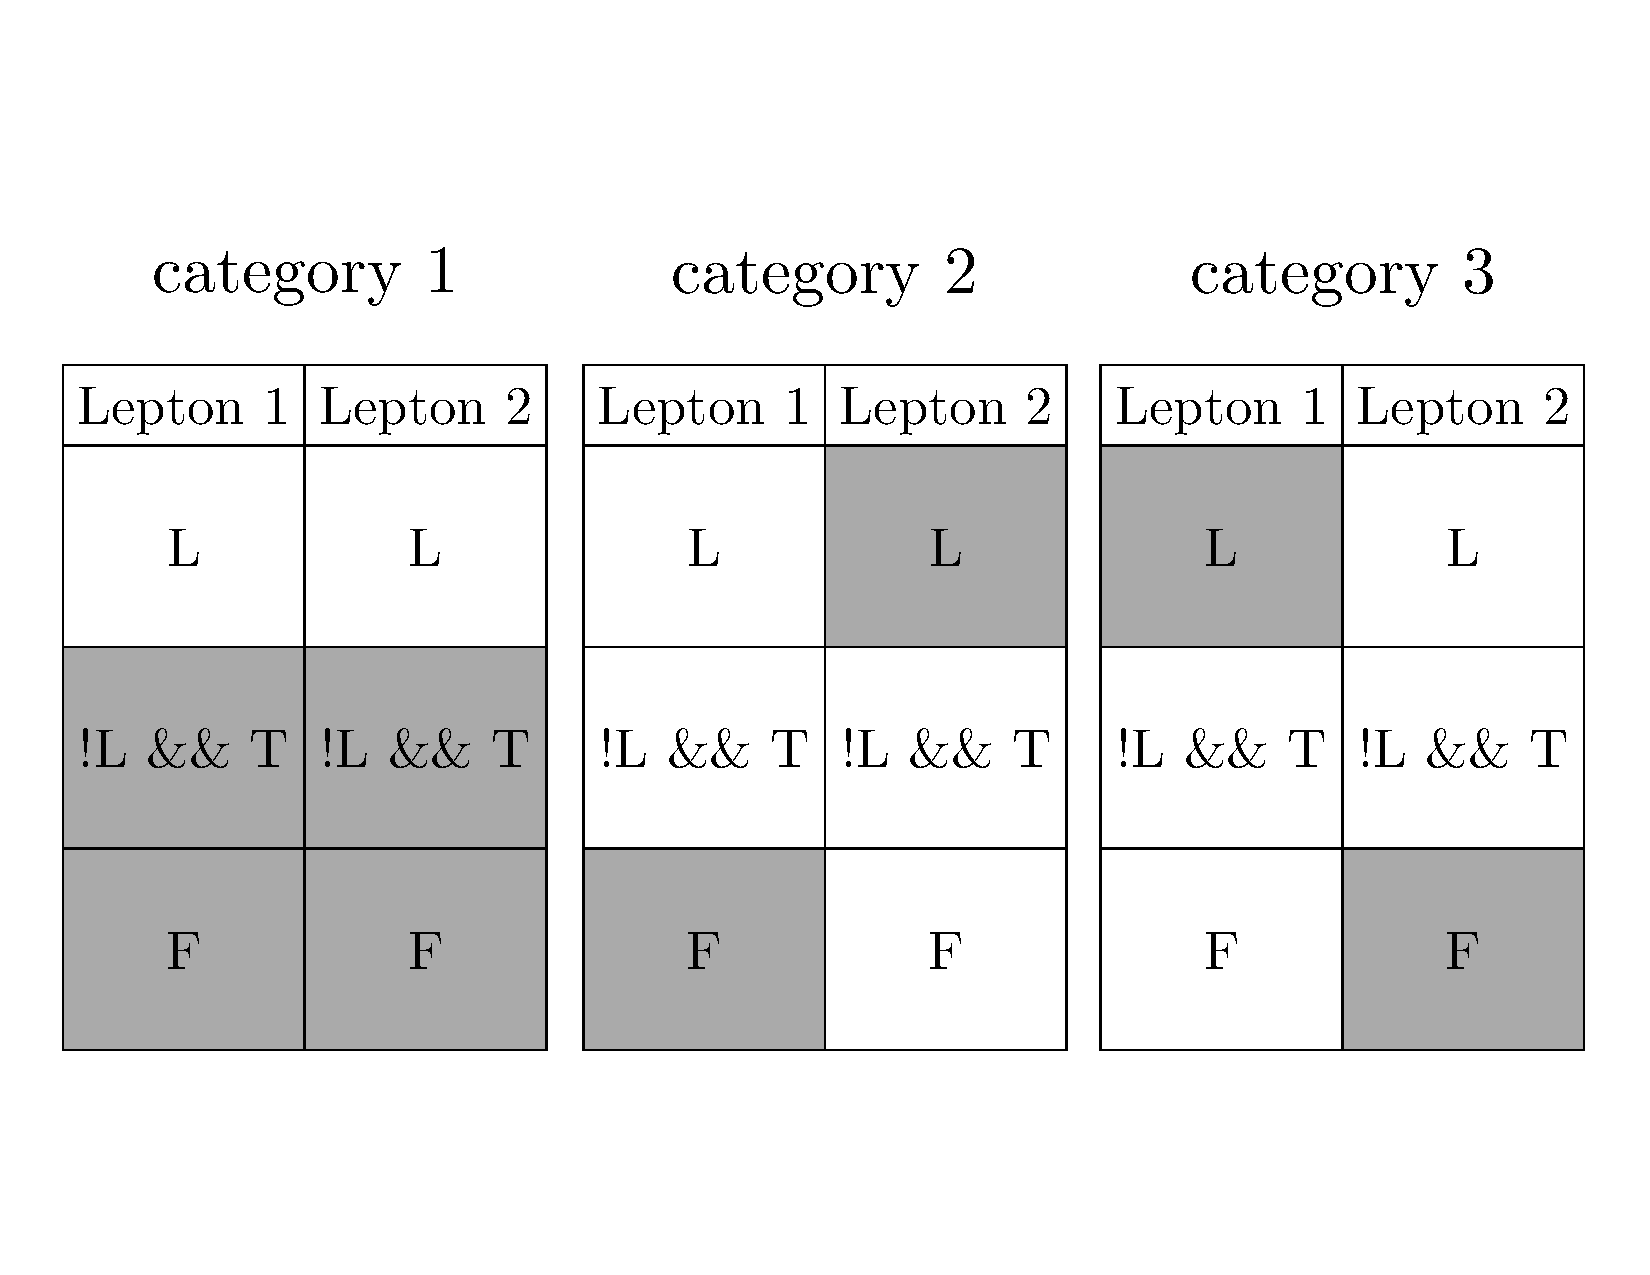
\includegraphics[width=0.8\textwidth]{figures/TriggerEfficiencyDiagram.pdf}
\caption{ Diagrams for the cases where double-lepton triggers fail. Lepton1(2) 
denotes offline leptons. L means leading leg requirement of double-lepton trigger. 
T means trailing leg requirement of double-lepton trigger. F means failing of 
trailing lepton requirement, thus leading lepton requirmement,of double-lepton trigger.
Shade means that the correponding offline lepton falls into that online requirement.}
\label{fig:trg_eff_diagram}
\end{figure*}
% Table version of the figure, figures/TriggerEfficiencyDiagram.pdf
%\begin{table}[htp]
%\begin{center}
%\begin{tabular}{ccc}
%\vspace{0.5cm}
%\textbf{category 1} & \textbf{category 2} & \textbf{category 3}  \\
%    \begin{tabular}{|c|c|}
%        \hline 
%        Lepton 1 & Lepton2 \\
%        \hline \hline 
%        L & L \\
%        \hline 
%        \underline{\textbf{!L AND T}} & \underline{\textbf{!L AND T}} \\
%        \hline 
%        \underline{\textbf{F}} & \underline{\textbf{F}} \\
%        \hline 
%    \end{tabular} 
%    &
%    \begin{tabular}{|c|c|}
%        \hline 
%        Lepton 1 & Lepton2 \\
%        \hline \hline 
%        L & \underline{\textbf{L}} \\
%        \hline 
%        !L AND T & !L AND T \\
%        \hline 
%        \underline{\textbf{F}} & F \\
%        \hline 
%    \end{tabular}  
%    &
%    \begin{tabular}{|c|c|}
%        \hline 
%        Lepton 1 & Lepton2 \\
%        \hline \hline 
%        \underline{\textbf{L}} & L \\
%        \hline 
%        !L AND T & !L AND T \\
%        \hline 
%        F & \underline{\textbf{F}} \\
%        \hline 
%    \end{tabular} 
%\end{tabular}
%\end{center}
%\end{table}
Figure \ref{fig:trg_eff_diagram} shows the failing cases of double-lepton trigger. 
There are three online cases for each lepton, which are passing leading leg requirement(L), 
passing trailing lepton requirement(T), and passing none of them(F). Shaded boxes 
show that each lepton falls into that category of offline requirement.   
There are 9($3\times3$) possible combinations in total, of which there are 6 cases 
that the trigger fails. Category 1(4 combinations) is the case where none of the 
two leptons pass leading leg requirement. Category 2 and 3 are the cases where one 
lepton passes leading leg requirement but the other leg fails trailing leg requirement.  
Converting this into equations, we have 
\begin{eqnarray} 
\label{eq:doubletrgeff}
\epsilon_{double-lepton} \left( p_{T1},\eta_1,p_{T2},\eta_2 \right)
&=&    
1 - \Big[   \\ 
& & 
\underbrace{
\left(1 - \epsilon_{DL}\left(p_{T1}, \eta_1\right)\right)
\left(1 - \epsilon_{DL}\left(p_{T2}, \eta_2\right)\right)  
}_\text{catetory 1} \\
& & 
+ \underbrace{
\epsilon_{DL}\left(p_{T2}, \eta_2\right)\left(1 - \epsilon_{DT}\left(p_{T1}, \eta_1\right)\right)
}_\text{catetory 2} \\
& &
+ \underbrace{
\epsilon_{DL}\left(p_{T1}, \eta_1\right)\left(1 - \epsilon_{DT}\left(p_{T2}, \eta_2\right)\right) 
}_\text{catetory 3}
\,\, \Big]
\end{eqnarray} 
where $p_{T1(2)} \textrm{ and } \eta_{1(2)}$ are \pt~and \Eta~of offline leptons, 
$\epsilon_{DL}$ is the efficiency for the leading leg of double-lepton trigger, 
and $\epsilon_{DT}$ is the efficiency for the trailng leg of double-lepton trigger. 
Each term corresponds to the 3 categories in Figure \ref{fig:trg_eff_diagram}.
In case the double-lepton trigger fails because one of the legs fails, the other leg 
which passed double-lepton trigger requirement might pass single lepton trigger. 
This way, inefficiency of double-lepton trigger can be recovered by single-lepton trigger.
The recovery of efficiency by single-lepton trigger is  
\begin{eqnarray} 
\label{eq:singletrgeff}
\epsilon_{single-lepton} \left( p_{T1},\eta_1,p_{T2},\eta_2 \right)
&=&    
\underbrace{
\left(1 - \epsilon_{DT}\left(p_{T1}, \eta_1\right)\right)
\epsilon_{S}\left(p_{T2}, \eta_2\right)  
}_\text{catetory 4} \\
& & 
+ \underbrace{
\left(1 - \epsilon_{DT}\left(p_{T2}, \eta_2\right)\right)
\epsilon_{S}\left(p_{T1}, \eta_1\right)  
}_\text{catetory 5} 
\end{eqnarray}
where $\epsilon_{S}$ is the efficiency of single-lepton trigger. 
Therefore, the total per-event trigger efficiency is given by 
\begin{eqnarray} 
\label{eq:doubletrgeff}
\epsilon_{event} \left( p_{T1},\eta_1,p_{T2},\eta_2 \right)
&=&    
1 - \Big[    
\left(1 - \epsilon_{DL}\left(p_{T1}, \eta_1\right)\right)
\left(1 - \epsilon_{DL}\left(p_{T2}, \eta_2\right)\right)  \\ 
& & 
+ \epsilon_{DL}\left(p_{T2}, \eta_2\right)\left(1 - \epsilon_{DT}\left(p_{T1}, \eta_1\right)\right) \\
& &
+ \epsilon_{DL}\left(p_{T1}, \eta_1\right)\left(1 - \epsilon_{DT}\left(p_{T2}, \eta_2\right)\right)  
\Big] \\
& &
+ \left(1 - \epsilon_{DT}\left(p_{T1}, \eta_1\right)\right)
\epsilon_{S}\left(p_{T2}, \eta_2\right)  \\ 
& & 
+ \left(1 - \epsilon_{DT}\left(p_{T2}, \eta_2\right)\right)
\epsilon_{S}\left(p_{T1}, \eta_1\right)  
\end{eqnarray} 

%%%% 
\begin{table}[!htp]
\begin{center}
\begin{tabular}{c|c|c|c|c}
\hline & $0 < |\eta| < 0.8$ & $0.8 < |\eta| < 1.479$ & $1.479 < |\eta| < 2$ & $2 < |\eta| < 2.5$  \\
\hline
$ 10 < p_T < 12.5$ & $1.0000 \pm 0.0045$ & $0.9946 \pm 0.0043$ & $0.9853 \pm 0.0191$ & $0.9724 \pm 0.0213$  \\
$12.5 < p_T <  15$ & $1.0000 \pm 0.0011$ & $0.9934 \pm 0.0024$ & $1.0000 \pm 0.0036$ & $0.9773 \pm 0.0095$  \\
$ 15 < p_T < 17.5$ & $0.9982 \pm 0.0010$ & $0.9971 \pm 0.0011$ & $0.9949 \pm 0.0030$ & $0.9886 \pm 0.0048$  \\
$17.5 < p_T <  20$ & $0.9990 \pm 0.0005$ & $0.9969 \pm 0.0008$ & $0.9952 \pm 0.0020$ & $0.9884 \pm 0.0034$  \\
$ 20 < p_T < 22.5$ & $0.9993 \pm 0.0004$ & $0.9980 \pm 0.0006$ & $0.9970 \pm 0.0012$ & $0.9873 \pm 0.0024$  \\
$22.5 < p_T <  25$ & $0.9997 \pm 0.0002$ & $0.9980 \pm 0.0004$ & $0.9962 \pm 0.0010$ & $0.9911 \pm 0.0016$  \\
$ 25 < p_T < 27.5$ & $0.9994 \pm 0.0002$ & $0.9982 \pm 0.0003$ & $0.9965 \pm 0.0007$ & $0.9905 \pm 0.0013$  \\
$27.5 < p_T <  30$ & $0.9993 \pm 0.0001$ & $0.9985 \pm 0.0002$ & $0.9975 \pm 0.0005$ & $0.9908 \pm 0.0011$  \\
$ 30 < p_T <  35$ & $0.9995 \pm 0.0001$ & $0.9986 \pm 0.0001$ & $0.9972 \pm 0.0003$ & $0.9920 \pm 0.0005$  \\
$ 35 < p_T <  40$ & $0.9996 \pm 0.0000$ & $0.9987 \pm 0.0001$ & $0.9972 \pm 0.0002$ & $0.9921 \pm 0.0004$  \\
$ 40 < p_T <  50$ & $0.9997 \pm 0.0000$ & $0.9990 \pm 0.0000$ & $0.9973 \pm 0.0001$ & $0.9925 \pm 0.0003$  \\
$ 50 < p_T < 7000$ & $0.9997 \pm 0.0000$ & $0.9992 \pm 0.0001$ & $0.9978 \pm 0.0002$ & $0.9922 \pm 0.0005$  \\
\hline
\end{tabular}
\caption{HWW Electron V00-02-09 Moriond jae NM1Eff TrigDzDbl}
\label{tab:trg_electron_dzdbl}
\end{center}
\end{table}
%
\begin{table}[!htp]
\begin{center}
\begin{tabular}{c|c|c|c|c}
\hline & $0 < |\eta| < 0.8$ & $0.8 < |\eta| < 1.479$ & $1.479 < |\eta| < 2$ & $2 < |\eta| < 2.5$  \\
\hline
$ 10 < p_T < 12.5$ & $0.0000 \pm 0.0041$ & $0.0000 \pm 0.0021$ & $0.0000 \pm 0.0102$ & $0.0000 \pm 0.0112$  \\
$12.5 < p_T <  15$ & $0.0000 \pm 0.0011$ & $0.0000 \pm 0.0009$ & $0.0092 \pm 0.0062$ & $0.0021 \pm 0.0049$  \\
$ 15 < p_T < 17.5$ & $0.0437 \pm 0.0035$ & $0.0460 \pm 0.0034$ & $0.2456 \pm 0.0128$ & $0.2300 \pm 0.0148$  \\
$17.5 < p_T <  20$ & $0.8312 \pm 0.0044$ & $0.6617 \pm 0.0057$ & $0.8570 \pm 0.0080$ & $0.8365 \pm 0.0098$  \\
$ 20 < p_T < 22.5$ & $0.9618 \pm 0.0019$ & $0.9560 \pm 0.0021$ & $0.9768 \pm 0.0027$ & $0.9685 \pm 0.0035$  \\
$22.5 < p_T <  25$ & $0.9709 \pm 0.0013$ & $0.9721 \pm 0.0014$ & $0.9843 \pm 0.0018$ & $0.9785 \pm 0.0024$  \\
$ 25 < p_T < 27.5$ & $0.9784 \pm 0.0009$ & $0.9764 \pm 0.0010$ & $0.9879 \pm 0.0013$ & $0.9859 \pm 0.0016$  \\
$27.5 < p_T <  30$ & $0.9823 \pm 0.0006$ & $0.9809 \pm 0.0008$ & $0.9884 \pm 0.0010$ & $0.9869 \pm 0.0012$  \\
$ 30 < p_T <  35$ & $0.9849 \pm 0.0003$ & $0.9842 \pm 0.0004$ & $0.9901 \pm 0.0005$ & $0.9869 \pm 0.0006$  \\
$ 35 < p_T <  40$ & $0.9880 \pm 0.0002$ & $0.9863 \pm 0.0003$ & $0.9925 \pm 0.0003$ & $0.9907 \pm 0.0004$  \\
$ 40 < p_T <  50$ & $0.9900 \pm 0.0001$ & $0.9903 \pm 0.0001$ & $0.9945 \pm 0.0002$ & $0.9912 \pm 0.0003$  \\
$ 50 < p_T < 7000$ & $0.9910 \pm 0.0002$ & $0.9925 \pm 0.0002$ & $0.9958 \pm 0.0003$ & $0.9911 \pm 0.0005$  \\
\hline
\end{tabular}
\caption{HWW Electron V00-02-09 Moriond jae NM1Eff TrigLeadDbl}
\label{tab:trg_electron_leaddbl}
\end{center}
\end{table}

%
\begin{table}[!htp]
\begin{center}
\begin{tabular}{c|c|c|c|c}
\hline & $0 < |\eta| < 0.8$ & $0.8 < |\eta| < 1.479$ & $1.479 < |\eta| < 2$ & $2 < |\eta| < 2.5$  \\
\hline
$ 10 < p_T < 12.5$ & $0.9101 \pm 0.0157$ & $0.8313 \pm 0.0135$ & $0.7598 \pm 0.0362$ & $0.8841 \pm 0.0306$  \\
$12.5 < p_T <  15$ & $0.9633 \pm 0.0051$ & $0.9284 \pm 0.0060$ & $0.9316 \pm 0.0126$ & $0.9382 \pm 0.0132$  \\
$ 15 < p_T < 17.5$ & $0.9685 \pm 0.0030$ & $0.9554 \pm 0.0034$ & $0.9572 \pm 0.0066$ & $0.9595 \pm 0.0076$  \\
$17.5 < p_T <  20$ & $0.9673 \pm 0.0022$ & $0.9665 \pm 0.0023$ & $0.9716 \pm 0.0041$ & $0.9774 \pm 0.0044$  \\
$ 20 < p_T < 22.5$ & $0.9695 \pm 0.0017$ & $0.9699 \pm 0.0018$ & $0.9762 \pm 0.0028$ & $0.9786 \pm 0.0030$  \\
$22.5 < p_T <  25$ & $0.9731 \pm 0.0012$ & $0.9745 \pm 0.0013$ & $0.9764 \pm 0.0021$ & $0.9758 \pm 0.0025$  \\
$ 25 < p_T < 27.5$ & $0.9771 \pm 0.0009$ & $0.9779 \pm 0.0010$ & $0.9831 \pm 0.0015$ & $0.9831 \pm 0.0017$  \\
$27.5 < p_T <  30$ & $0.9810 \pm 0.0007$ & $0.9807 \pm 0.0008$ & $0.9829 \pm 0.0012$ & $0.9842 \pm 0.0013$  \\
$ 30 < p_T <  35$ & $0.9828 \pm 0.0003$ & $0.9831 \pm 0.0004$ & $0.9830 \pm 0.0006$ & $0.9840 \pm 0.0007$  \\
$ 35 < p_T <  40$ & $0.9850 \pm 0.0002$ & $0.9843 \pm 0.0003$ & $0.9861 \pm 0.0004$ & $0.9879 \pm 0.0005$  \\
$ 40 < p_T <  50$ & $0.9870 \pm 0.0001$ & $0.9874 \pm 0.0002$ & $0.9883 \pm 0.0002$ & $0.9885 \pm 0.0003$  \\
$ 50 < p_T < 7000$ & $0.9882 \pm 0.0003$ & $0.9893 \pm 0.0003$ & $0.9900 \pm 0.0004$ & $0.9888 \pm 0.0006$  \\
\hline
\end{tabular}
\caption{HWW Electron V00-02-09 Moriond jae NM1Eff TrigTrailDbl}
\label{tab:trg_electron_traildbl}
\end{center}
\end{table}

%
\begin{table}[!htp]
\begin{center}
\begin{tabular}{c|c|c|c|c}
\hline & $0 < |\eta| < 0.8$ & $0.8 < |\eta| < 1.479$ & $1.479 < |\eta| < 2$ & $2 < |\eta| < 2.5$  \\
\hline
$ 10 < p_T < 12.5$ & $0.0000 \pm 0.0021$ & $0.0000 \pm 0.0010$ & $0.0000 \pm 0.0051$ & $0.0000 \pm 0.0057$  \\
$12.5 < p_T <  15$ & $0.0000 \pm 0.0005$ & $0.0000 \pm 0.0004$ & $0.0000 \pm 0.0017$ & $0.0000 \pm 0.0020$  \\
$ 15 < p_T < 17.5$ & $0.0000 \pm 0.0002$ & $0.0000 \pm 0.0002$ & $0.0000 \pm 0.0008$ & $0.0000 \pm 0.0010$  \\
$17.5 < p_T <  20$ & $0.0000 \pm 0.0001$ & $0.0000 \pm 0.0001$ & $0.0002 \pm 0.0005$ & $0.0000 \pm 0.0006$  \\
$ 20 < p_T < 22.5$ & $0.0000 \pm 0.0001$ & $0.0000 \pm 0.0001$ & $0.0005 \pm 0.0004$ & $0.0007 \pm 0.0005$  \\
$22.5 < p_T <  25$ & $0.0006 \pm 0.0002$ & $0.0006 \pm 0.0002$ & $0.0118 \pm 0.0011$ & $0.0250 \pm 0.0018$  \\
$ 25 < p_T < 27.5$ & $0.0255 \pm 0.0007$ & $0.0251 \pm 0.0007$ & $0.1320 \pm 0.0026$ & $0.1636 \pm 0.0032$  \\
$27.5 < p_T <  30$ & $0.6009 \pm 0.0016$ & $0.4072 \pm 0.0018$ & $0.4926 \pm 0.0031$ & $0.4710 \pm 0.0035$  \\
$ 30 < p_T <  35$ & $0.8905 \pm 0.0005$ & $0.8634 \pm 0.0007$ & $0.6775 \pm 0.0015$ & $0.6602 \pm 0.0018$  \\
$ 35 < p_T <  40$ & $0.9171 \pm 0.0004$ & $0.9012 \pm 0.0004$ & $0.7285 \pm 0.0011$ & $0.7103 \pm 0.0013$  \\
$ 40 < p_T <  50$ & $0.9361 \pm 0.0002$ & $0.9239 \pm 0.0003$ & $0.7618 \pm 0.0007$ & $0.7298 \pm 0.0009$  \\
$ 50 < p_T < 7000$ & $0.9471 \pm 0.0004$ & $0.9402 \pm 0.0005$ & $0.7808 \pm 0.0012$ & $0.7374 \pm 0.0017$  \\
\hline
\end{tabular}
\caption{HWW Electron V00-02-09 Moriond jae NM1Eff TrigSgl}
\label{tab:trg_electron_sgl}
\end{center}
\end{table}

The efficiency of dZ, leading and trailing leg requirements for double-electron triggers is shown in 
Table \ref{tab:trg_electron_dzdbl} - \ref{tab:trg_electron_traildbl}. 
The efficiency of single-electron trigger is shown in \ref{tab:trg_electron_sgl}. 

%
\begin{table}[!htp]
\begin{center}
\begin{tabular}{c|c|c|c|c}
\hline & $0 < |\eta| < 0.8$ & $0.8 < |\eta| < 1.2$ & $1.2 < |\eta| < 2.1$ & $2.1 < |\eta| < 2.4$  \\
\hline
$ 10 < p_T < 12.5$ & $0.9710 \pm 0.0045$ & $0.9687 \pm 0.0045$ & $0.9572 \pm 0.0029$ & $0.9682 \pm 0.0044$  \\
$12.5 < p_T <  15$ & $0.9714 \pm 0.0028$ & $0.9692 \pm 0.0032$ & $0.9612 \pm 0.0022$ & $0.9617 \pm 0.0040$  \\
$ 15 < p_T < 17.5$ & $0.9794 \pm 0.0017$ & $0.9702 \pm 0.0026$ & $0.9710 \pm 0.0016$ & $0.9688 \pm 0.0031$  \\
$17.5 < p_T <  20$ & $0.9907 \pm 0.0009$ & $0.9838 \pm 0.0016$ & $0.9819 \pm 0.0011$ & $0.9764 \pm 0.0023$  \\
$ 20 < p_T < 22.5$ & $0.9912 \pm 0.0007$ & $0.9862 \pm 0.0012$ & $0.9823 \pm 0.0009$ & $0.9755 \pm 0.0020$  \\
$22.5 < p_T <  25$ & $0.9896 \pm 0.0006$ & $0.9873 \pm 0.0009$ & $0.9828 \pm 0.0007$ & $0.9785 \pm 0.0016$  \\
$ 25 < p_T < 27.5$ & $0.9897 \pm 0.0005$ & $0.9886 \pm 0.0007$ & $0.9815 \pm 0.0006$ & $0.9784 \pm 0.0014$  \\
$27.5 < p_T <  30$ & $0.9900 \pm 0.0004$ & $0.9874 \pm 0.0006$ & $0.9813 \pm 0.0005$ & $0.9794 \pm 0.0011$  \\
$ 30 < p_T <  35$ & $0.9911 \pm 0.0002$ & $0.9869 \pm 0.0004$ & $0.9810 \pm 0.0003$ & $0.9805 \pm 0.0006$  \\
$ 35 < p_T <  40$ & $0.9918 \pm 0.0001$ & $0.9862 \pm 0.0003$ & $0.9790 \pm 0.0003$ & $0.9789 \pm 0.0006$  \\
$ 40 < p_T <  50$ & $0.9934 \pm 0.0001$ & $0.9855 \pm 0.0002$ & $0.9767 \pm 0.0002$ & $0.9777 \pm 0.0004$  \\
$ 50 < p_T < 7000$ & $0.9937 \pm 0.0002$ & $0.9855 \pm 0.0003$ & $0.9747 \pm 0.0004$ & $0.9799 \pm 0.0009$  \\
\hline
\end{tabular}
\caption{HWW Muon V00-02-09 Moriond jae NM1Eff TrigDzDbl}
\label{tab:trg_muon_dzdbl}
\end{center}
\end{table}

\begin{table}[!htp]
\begin{center}
\begin{tabular}{c|c|c|c|c}
\hline & $0 < |\eta| < 0.8$ & $0.8 < |\eta| < 1.2$ & $1.2 < |\eta| < 2.1$ & $2.1 < |\eta| < 2.4$  \\
\hline
$ 10 < p_T < 12.5$ & $0.0005 \pm 0.0012$ & $0.0114 \pm 0.0030$ & $0.0034 \pm 0.0010$ & $0.0085 \pm 0.0025$  \\
$12.5 < p_T <  15$ & $0.0005 \pm 0.0006$ & $0.0188 \pm 0.0026$ & $0.0068 \pm 0.0010$ & $0.0092 \pm 0.0021$  \\
$ 15 < p_T < 17.5$ & $0.2500 \pm 0.0049$ & $0.2363 \pm 0.0060$ & $0.2688 \pm 0.0040$ & $0.2442 \pm 0.0069$  \\
$17.5 < p_T <  20$ & $0.9696 \pm 0.0015$ & $0.9169 \pm 0.0033$ & $0.9036 \pm 0.0023$ & $0.8007 \pm 0.0055$  \\
$ 20 < p_T < 22.5$ & $0.9714 \pm 0.0011$ & $0.9243 \pm 0.0026$ & $0.9138 \pm 0.0018$ & $0.8176 \pm 0.0046$  \\
$22.5 < p_T <  25$ & $0.9717 \pm 0.0009$ & $0.9269 \pm 0.0021$ & $0.9236 \pm 0.0015$ & $0.8479 \pm 0.0037$  \\
$ 25 < p_T < 27.5$ & $0.9717 \pm 0.0007$ & $0.9311 \pm 0.0017$ & $0.9221 \pm 0.0012$ & $0.8506 \pm 0.0031$  \\
$27.5 < p_T <  30$ & $0.9712 \pm 0.0006$ & $0.9280 \pm 0.0014$ & $0.9233 \pm 0.0010$ & $0.8558 \pm 0.0026$  \\
$ 30 < p_T <  35$ & $0.9706 \pm 0.0003$ & $0.9289 \pm 0.0008$ & $0.9198 \pm 0.0006$ & $0.8692 \pm 0.0014$  \\
$ 35 < p_T <  40$ & $0.9722 \pm 0.0002$ & $0.9286 \pm 0.0006$ & $0.9206 \pm 0.0005$ & $0.8796 \pm 0.0012$  \\
$ 40 < p_T <  50$ & $0.9726 \pm 0.0002$ & $0.9320 \pm 0.0004$ & $0.9215 \pm 0.0003$ & $0.8889 \pm 0.0009$  \\
$ 50 < p_T < 7000$ & $0.9725 \pm 0.0003$ & $0.9337 \pm 0.0007$ & $0.9216 \pm 0.0006$ & $0.9016 \pm 0.0018$  \\
\hline
\end{tabular}
\caption{HWW Muon V00-02-09 Moriond jae NM1Eff TrigLeadDbl}
\label{tab:trg_muon_leaddbl}
\end{center}
\end{table}

\begin{table}[!htp]
\begin{center}
\begin{tabular}{c|c|c|c|c}
\hline & $0 < |\eta| < 0.8$ & $0.8 < |\eta| < 1.2$ & $1.2 < |\eta| < 2.1$ & $2.1 < |\eta| < 2.4$  \\
\hline
$ 10 < p_T < 12.5$ & $0.0000 \pm 0.0005$ & $0.0000 \pm 0.0005$ & $0.0001 \pm 0.0002$ & $0.0000 \pm 0.0004$  \\
$12.5 < p_T <  15$ & $0.0000 \pm 0.0002$ & $0.0001 \pm 0.0003$ & $0.0002 \pm 0.0002$ & $0.0000 \pm 0.0003$  \\
$ 15 < p_T < 17.5$ & $0.0000 \pm 0.0001$ & $0.0004 \pm 0.0003$ & $0.0001 \pm 0.0001$ & $0.0000 \pm 0.0002$  \\
$17.5 < p_T <  20$ & $0.0000 \pm 0.0001$ & $0.0015 \pm 0.0004$ & $0.0004 \pm 0.0001$ & $0.0000 \pm 0.0002$  \\
$ 20 < p_T < 22.5$ & $0.0004 \pm 0.0001$ & $0.0030 \pm 0.0004$ & $0.0028 \pm 0.0003$ & $0.0000 \pm 0.0001$  \\
$22.5 < p_T <  25$ & $0.4031 \pm 0.0018$ & $0.3699 \pm 0.0027$ & $0.3912 \pm 0.0019$ & $0.0000 \pm 0.0001$  \\
$ 25 < p_T < 27.5$ & $0.8847 \pm 0.0010$ & $0.8076 \pm 0.0018$ & $0.7733 \pm 0.0014$ & $0.0001 \pm 0.0001$  \\
$27.5 < p_T <  30$ & $0.8955 \pm 0.0008$ & $0.8172 \pm 0.0015$ & $0.7881 \pm 0.0011$ & $0.0002 \pm 0.0001$  \\
$ 30 < p_T <  35$ & $0.9100 \pm 0.0004$ & $0.8267 \pm 0.0008$ & $0.7968 \pm 0.0006$ & $0.0001 \pm 0.0000$  \\
$ 35 < p_T <  40$ & $0.9230 \pm 0.0003$ & $0.8368 \pm 0.0006$ & $0.8048 \pm 0.0005$ & $0.0001 \pm 0.0000$  \\
$ 40 < p_T <  50$ & $0.9350 \pm 0.0002$ & $0.8480 \pm 0.0004$ & $0.8161 \pm 0.0003$ & $0.0001 \pm 0.0000$  \\
$ 50 < p_T < 7000$ & $0.9408 \pm 0.0003$ & $0.8526 \pm 0.0007$ & $0.8207 \pm 0.0006$ & $0.0002 \pm 0.0001$  \\
\hline
\end{tabular}
\caption{HWW Muon V00-02-09 Moriond jae NM1Eff TrigSgl}
\label{tab:trg_muon_sgl}
\end{center}
\end{table}

\begin{table}[!htp]
\begin{center}
\begin{tabular}{c|c|c|c|c}
\hline & $0 < |\eta| < 0.8$ & $0.8 < |\eta| < 1.2$ & $1.2 < |\eta| < 2.1$ & $2.1 < |\eta| < 2.4$  \\
\hline
$ 10 < p_T < 12.5$ & $0.9838 \pm 0.0035$ & $0.9752 \pm 0.0041$ & $0.9779 \pm 0.0021$ & $0.9371 \pm 0.0057$  \\
$12.5 < p_T <  15$ & $0.9850 \pm 0.0021$ & $0.9735 \pm 0.0030$ & $0.9814 \pm 0.0016$ & $0.9403 \pm 0.0047$  \\
$ 15 < p_T < 17.5$ & $0.9846 \pm 0.0015$ & $0.9770 \pm 0.0023$ & $0.9817 \pm 0.0013$ & $0.9391 \pm 0.0040$  \\
$17.5 < p_T <  20$ & $0.9824 \pm 0.0012$ & $0.9772 \pm 0.0018$ & $0.9807 \pm 0.0011$ & $0.9422 \pm 0.0033$  \\
$ 20 < p_T < 22.5$ & $0.9831 \pm 0.0009$ & $0.9791 \pm 0.0014$ & $0.9812 \pm 0.0009$ & $0.9388 \pm 0.0029$  \\
$22.5 < p_T <  25$ & $0.9824 \pm 0.0007$ & $0.9782 \pm 0.0012$ & $0.9826 \pm 0.0007$ & $0.9468 \pm 0.0024$  \\
$ 25 < p_T < 27.5$ & $0.9837 \pm 0.0006$ & $0.9797 \pm 0.0010$ & $0.9822 \pm 0.0006$ & $0.9438 \pm 0.0020$  \\
$27.5 < p_T <  30$ & $0.9831 \pm 0.0005$ & $0.9792 \pm 0.0008$ & $0.9829 \pm 0.0005$ & $0.9440 \pm 0.0017$  \\
$ 30 < p_T <  35$ & $0.9827 \pm 0.0002$ & $0.9797 \pm 0.0004$ & $0.9814 \pm 0.0003$ & $0.9482 \pm 0.0010$  \\
$ 35 < p_T <  40$ & $0.9840 \pm 0.0002$ & $0.9792 \pm 0.0003$ & $0.9825 \pm 0.0002$ & $0.9501 \pm 0.0008$  \\
$ 40 < p_T <  50$ & $0.9846 \pm 0.0001$ & $0.9800 \pm 0.0002$ & $0.9831 \pm 0.0002$ & $0.9551 \pm 0.0006$  \\
$ 50 < p_T < 7000$ & $0.9851 \pm 0.0002$ & $0.9804 \pm 0.0004$ & $0.9829 \pm 0.0003$ & $0.9563 \pm 0.0013$  \\
\hline
\end{tabular}
\caption{HWW Muon V00-02-09 Moriond jae NM1Eff TrigTrailDbl}
\label{tab:trg_muon_traildbl}
\end{center}
\end{table}

The efficiency of dZ, leading and trailing leg requirements for double-muon triggers is shown in 
Table \ref{tab:trg_muon_dzdbl} - \ref{tab:trg_muon_traildbl}. 
The efficiency of single-muon trigger is shown in \ref{tab:trg_muon_sgl}. 


%%%%%%%%%%%%%%%%%%%%%%%%%%%%%%%%%%%%%%%%%%%%%%%%%%%%%%%%%%%%%%%%%%%%%%%%%%%%%%%%%%%%%%%%%%
\newpage
\section{Jet Counting Efficiency} 

The analysis is optimized for different categories of number of jets. 
But, jet counting efficiency which is defined as 
$\displaystyle  \epsilon_{0/1} = \frac{N_{njet=0/1}}{N_{njet\geq0}}$ 
can be different in simulation and data.  
So, we correct the efficiency of \hww~in MC by a data-to-MC scale 
factor measured in MC and data using \dyll~events.  
The jet counting efficiency of \hww~events,$\epsilon_{\hww}$, 
is calculated by 
\begin{eqnarray} 
\epsilon_{\hww} 
= \epsilon_{\hww}^{MC} \times \frac{\epsilon_{\dyll}^{Data}}{\epsilon_{\dyll}^{MC}}  
\end{eqnarray} 
where $\epsilon_{\hww}^{MC}$ is jet counting efficiency of \hww~in simulation, 
and $\frac{\epsilon_{\dyll}^{Data}}{\epsilon_{\dyll}^{MC}}$
is a data-to-simulation scale factor measured using \dyll~events.
The efficiencies of \dyll~events are evaluated using Drell-Yan events with  
dilepton mass within 7.5 GeV of the Z peak. 
%%%%%%%%%%%%%%%%%%%%%%%%%
\begin{figure}[!hbtp]
\centering
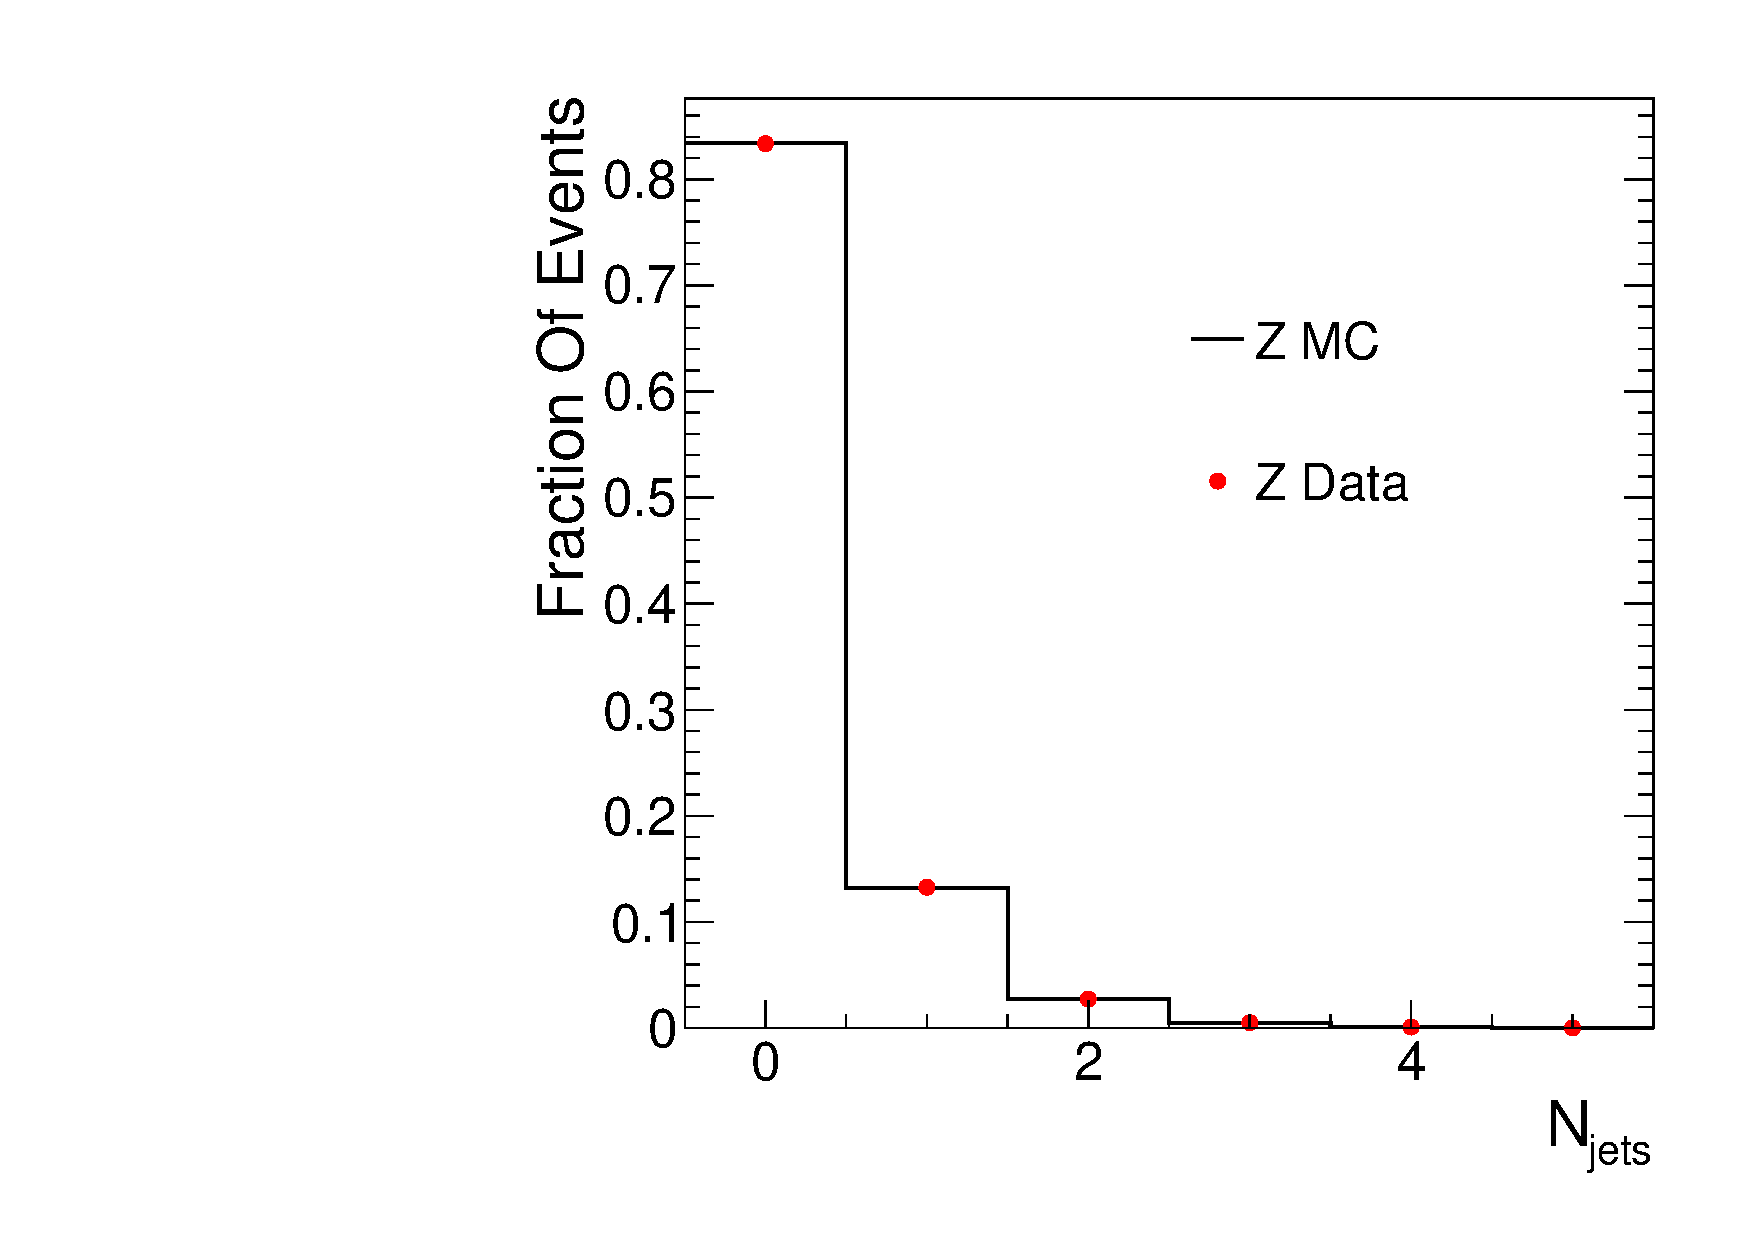
\includegraphics[width=.7\textwidth]{figures/Znjets.pdf}
\caption{The number of Jets observed in data (red solid dot) and MC (black line) for the Z events. }
\label{fig:znjets}
\end{figure}
%%%%%%%%%%%%%%%%%%%%%%%%%
\begin{figure}[!hbtp]
\centering
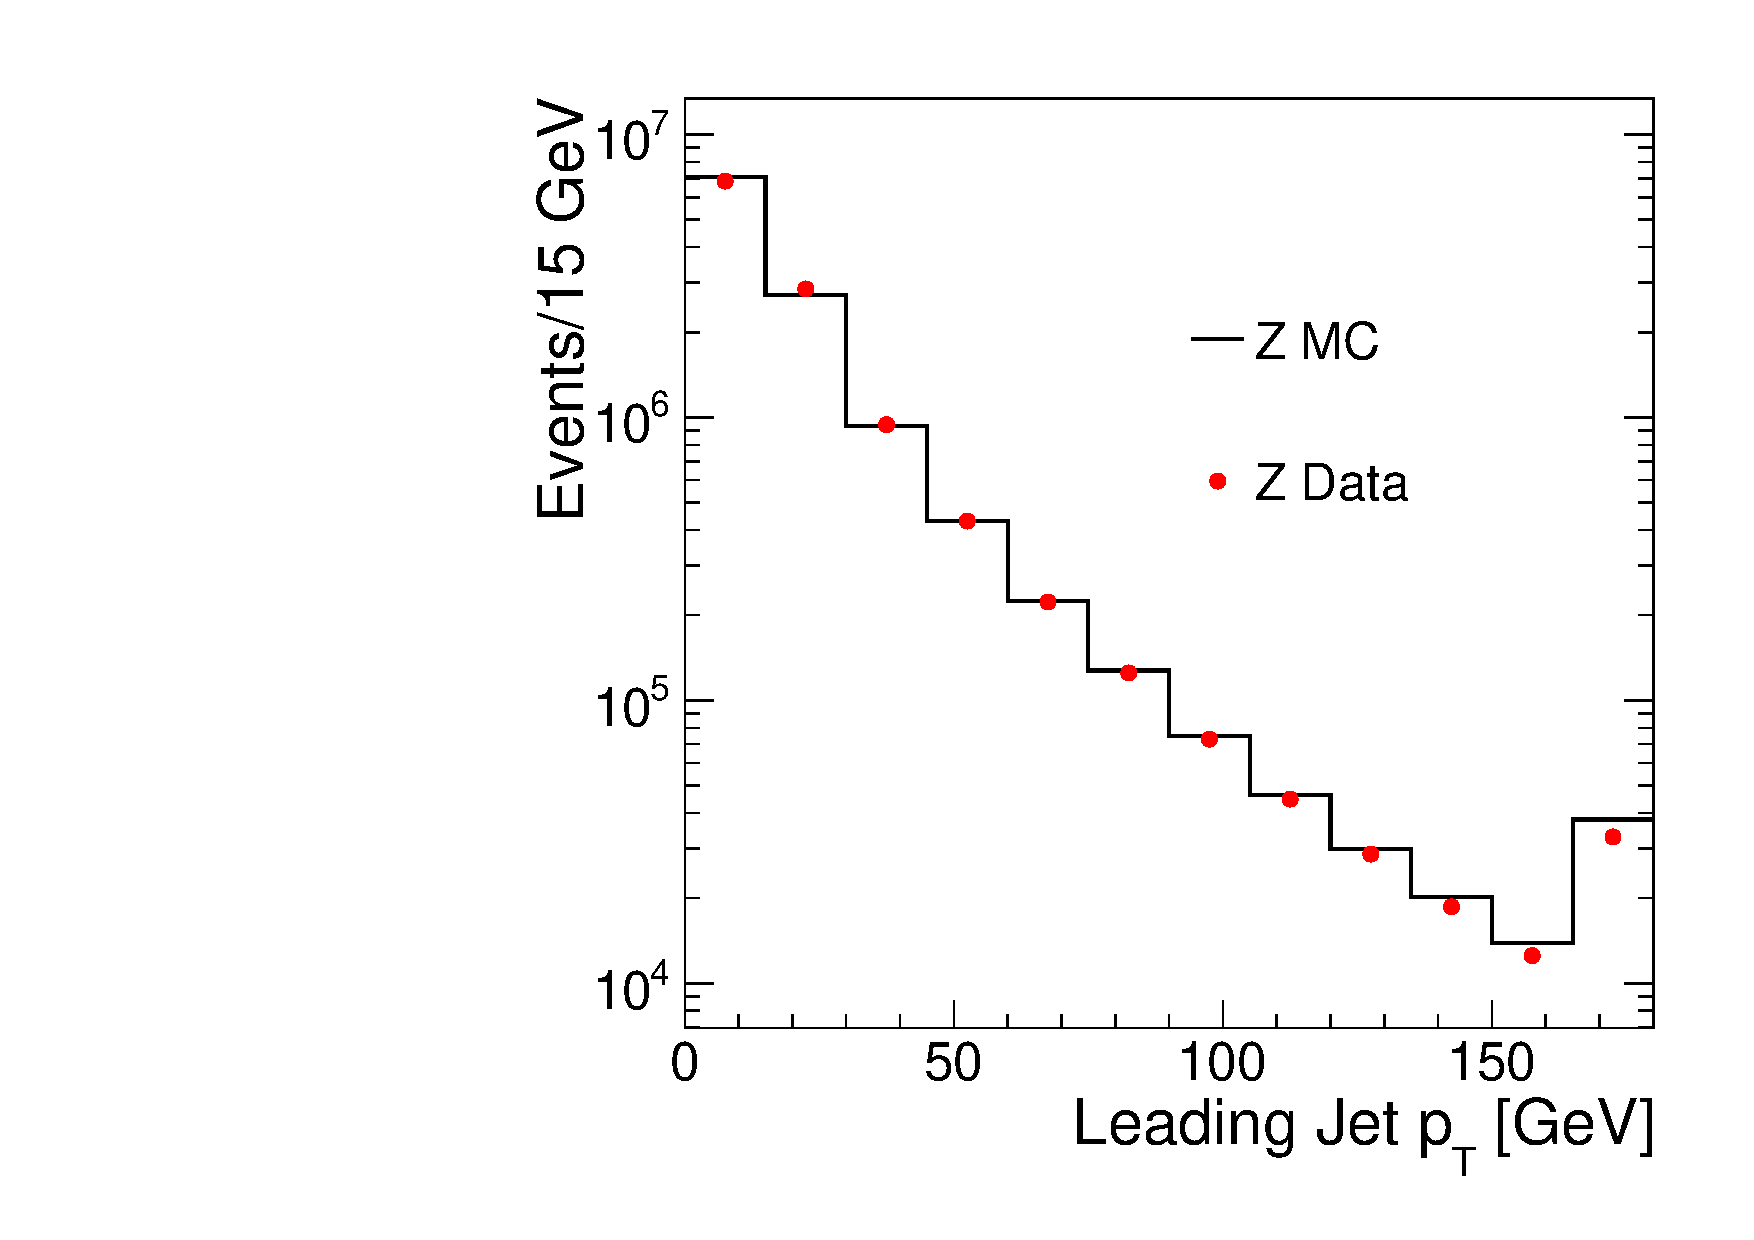
\includegraphics[width=.45\textwidth]{figures/ZjetpT.pdf}
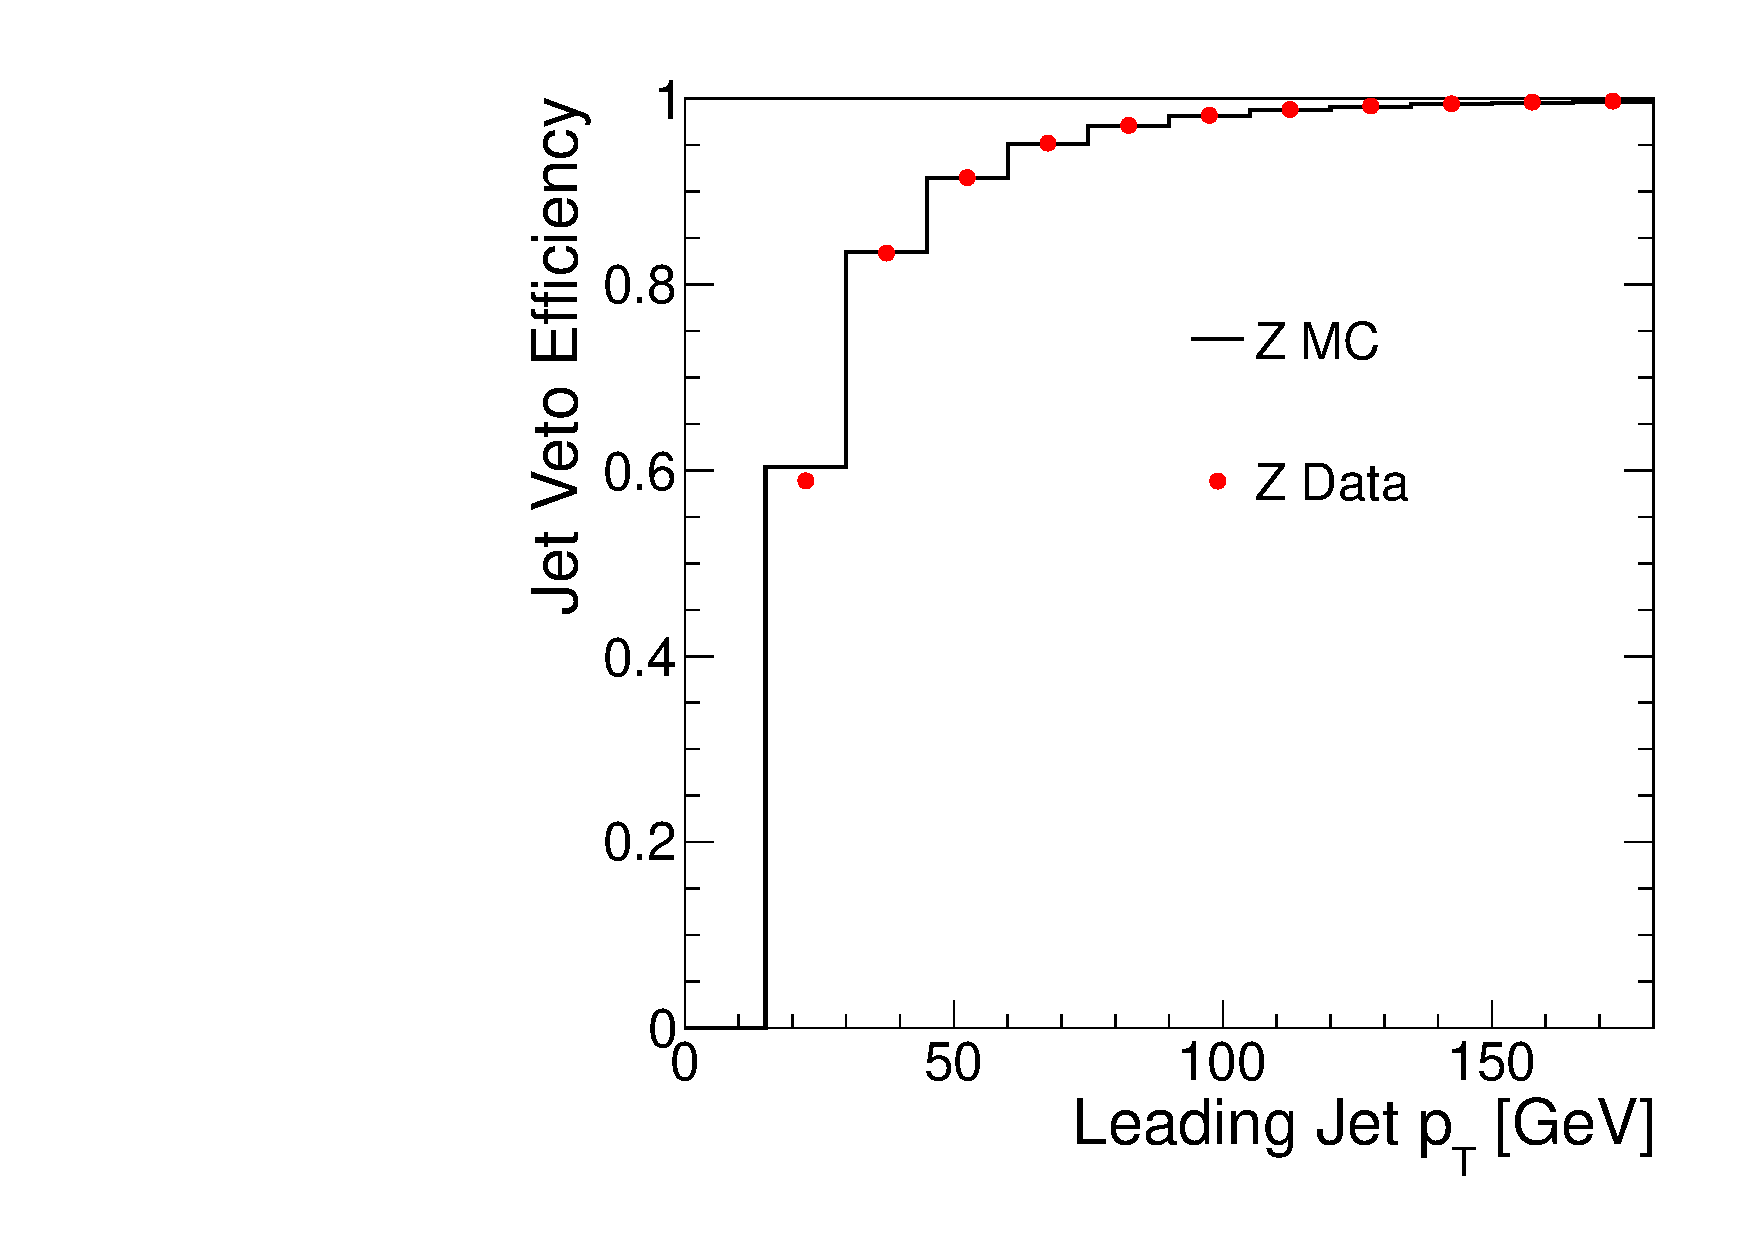
\includegraphics[width=.45\textwidth]{figures/Zjetvetoeff.pdf}
\caption{The leading jet $pT$ \subref{subfig:jetpt_z} and the jet veto efficiency as a function 
of the leading jet $p_T$ \subref{subfig:jetveto_z} in data (red solid dot) and MC (black line) for the Z events. }
\label{fig:jetveto_z}
\end{figure}
%%%%%%%%%%%%%%%%%%%%%%%%%
\begin{figure}[!hbtp]
\centering
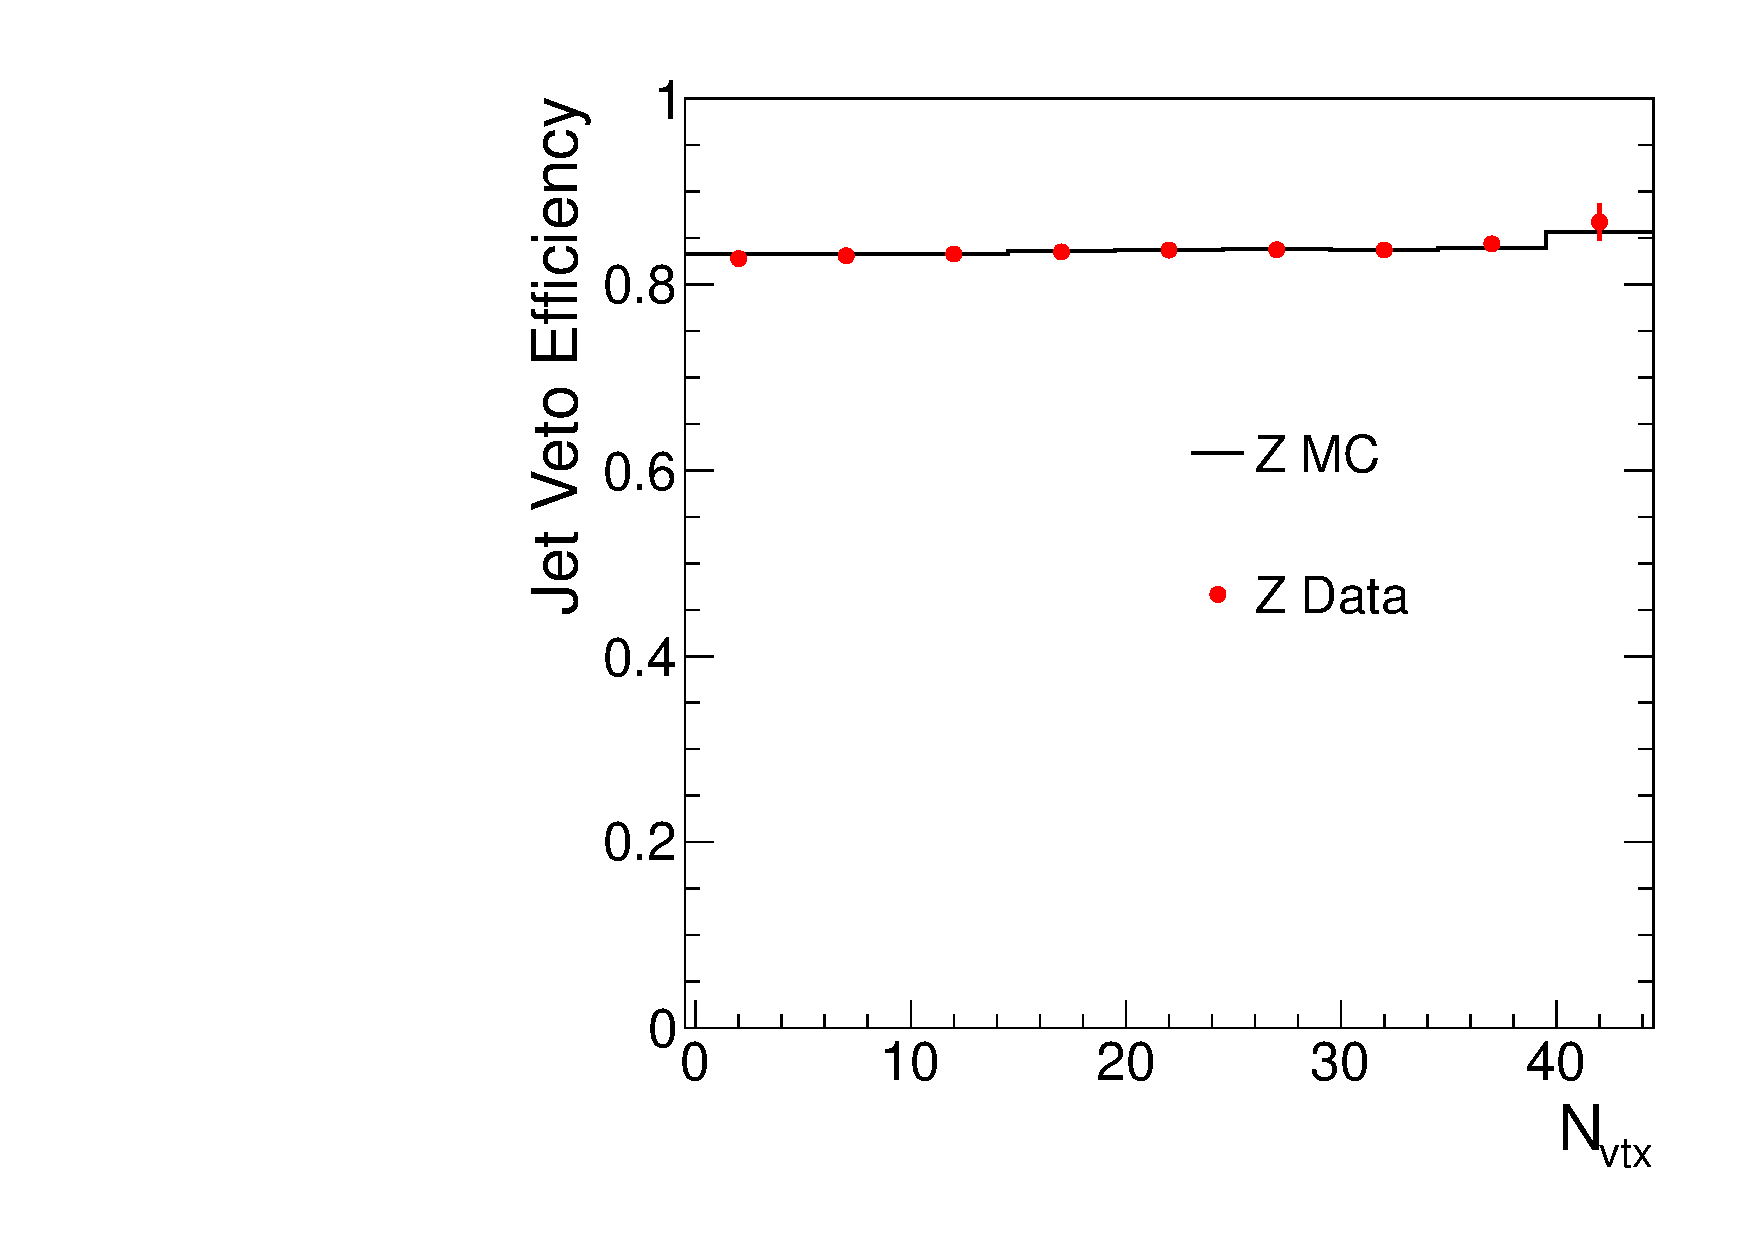
\includegraphics[width=.45\textwidth]{figures/Zjetvetoeff_vs_nvtx.pdf}
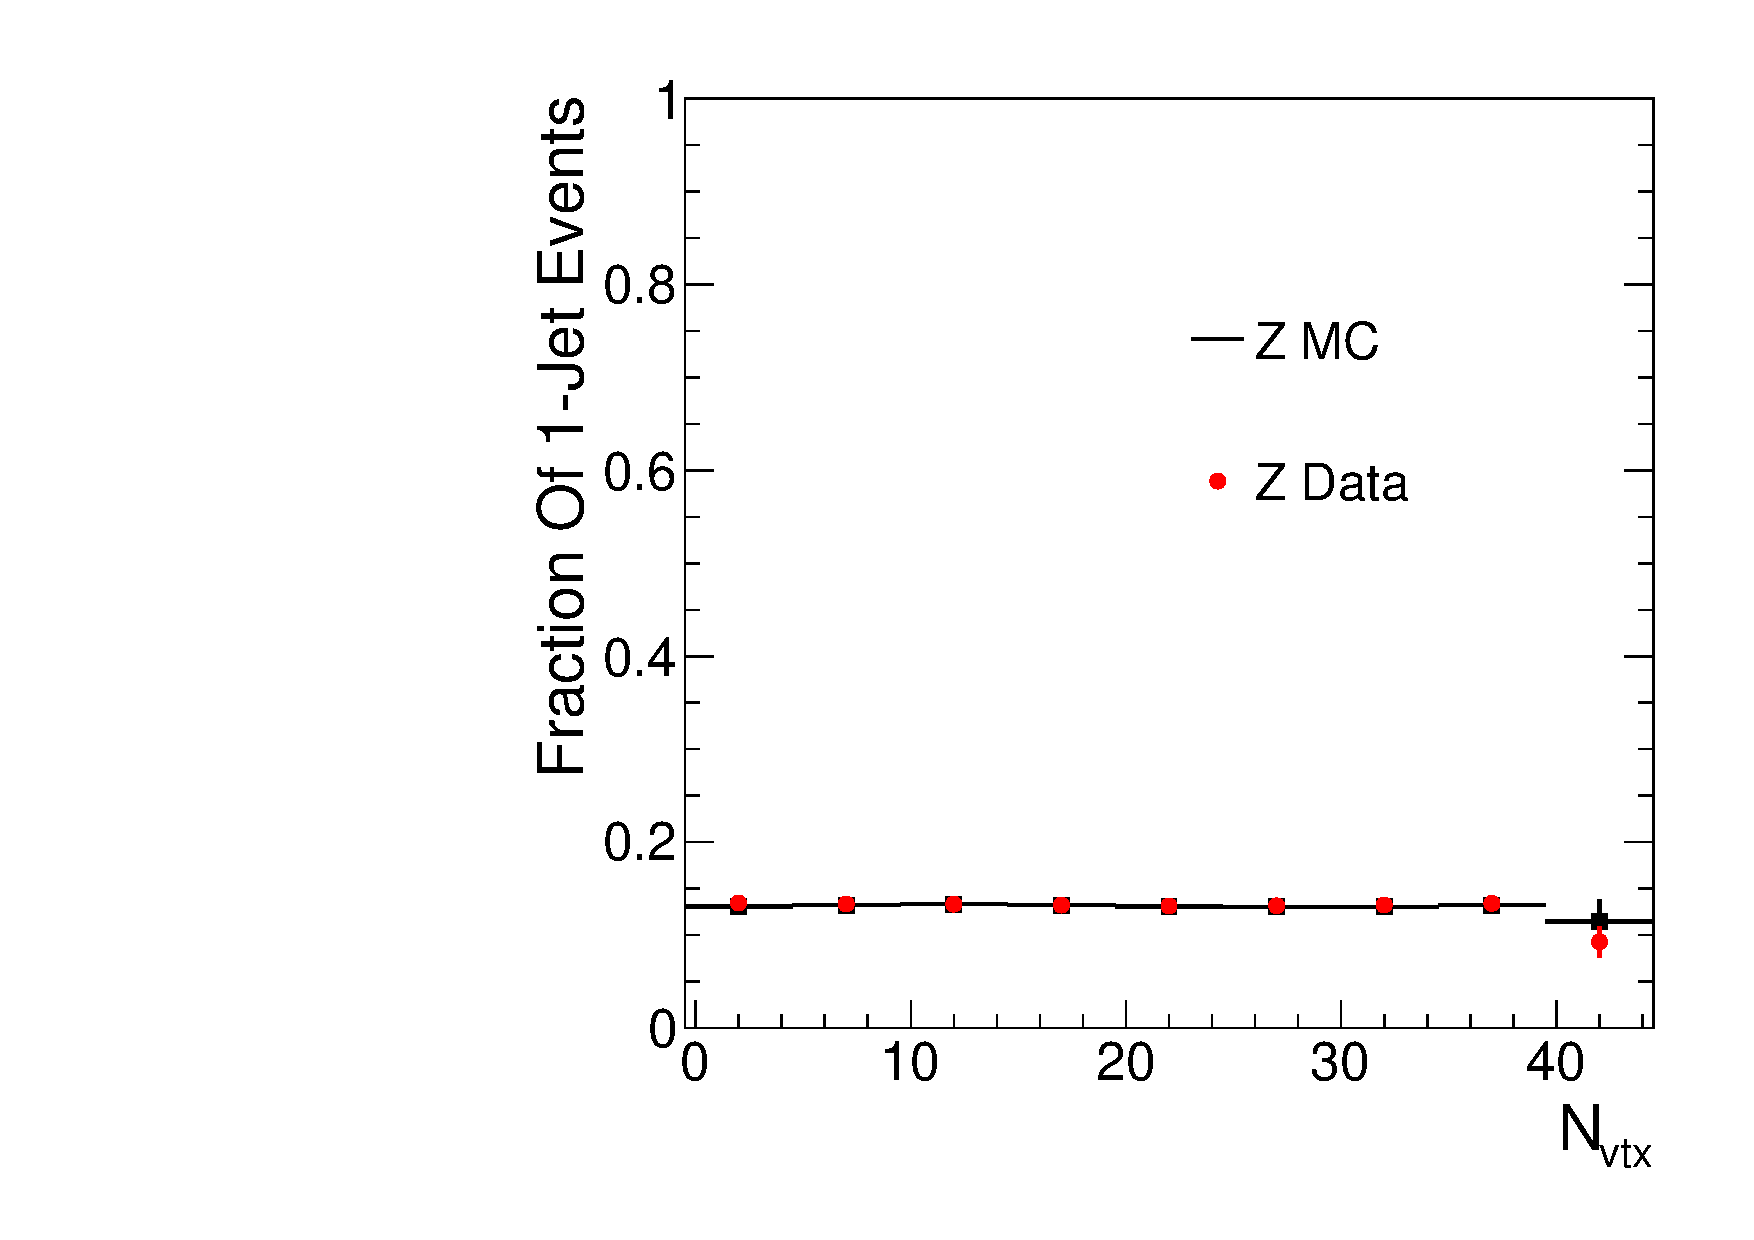
\includegraphics[width=.45\textwidth]{figures/Zonejeteff_vs_nvtx.pdf}
\caption{The fraction of events with 0 Jet \subref{subfig:zerojetfrac_z} and 1 Jet \subref{subfig:onejetfrac_z} 
as a function of the number of vertices, comparing data (red solid dot) and MC (black solid square) for the Z events. }
\label{fig:jetfrac_z}
\end{figure}
%%%%%%%%%%%%%%%%%%%%%%%%%

Figure \ref{fig:znjets} shows distribution of number of jets for data and MC. 
In all bins good agreement with difference less than 1\% is shown. 
The systematic uncertainty to jet counting efficiency comes from statistics 
when measuring data-to-MC scale factor and theoretical uncertainty of jet 
counting in \hww~simulation. The former is less than 1\% being negligible 
compared to theoretical uncertainty which is at the level of 15\%. 
This uncertainty will be discussed in the chapter for Systematic Uncertainty \ref{ch:systematics}. 

Figure \ref{fig:jetveto_z} shows \pt~distribution of leading jet (left) 
and jet veto effciency as a function of leading jet \pt(right)
With the jet \pt~threshold 30 \GeV, agreement between data and MC is very good. 
Figure \ref{fig:jetfrac_z} shows fraction of events with 0 jet and 
1 jet as a function of number of recontructed vertexes(Nvtx). 
Data and MC show very good agreement.
Dependence of efficiencies on Nvtx is small in both data and MC.
Thus, with the chosen jet idenfication, jet counting efficiency 
is not affected by reweighting by number of Pile-Up events. 
\textcolor{red}{(fix this sentence to read better)} 


